\chapter{Anatomía de la columna lumbar y los discos intervertebrales}
\label{anexo:anatomia-lumbar}

Este anexo resume las nociones anatómicas mínimas necesarias para comprender el dominio del prototipo. Está dirigido a lectores sin formación médica y no pretende ser exhaustivo desde el punto de vista clínico.

La columna vertebral es una estructura ósea que sostiene el tronco, permite el movimiento y protege la médula espinal. Se organiza en regiones; la región lumbar es la parte baja de la espalda y está formada por cinco vértebras, denominadas L1 a L5, ubicadas entre la columna torácica y el sacro. Por soportar gran parte del peso corporal y concentrar mucha movilidad, es una zona especialmente propensa al dolor y a la degeneración.

Cada vértebra está compuesta, a grandes rasgos, por un cuerpo vertebral anterior, de forma cilíndrica, que soporta la carga, y un arco posterior que rodea y protege el canal espinal. Las vértebras se apilan una sobre otra y, en conjunto, conforman el eje que da soporte al cuerpo.

Entre cada par de cuerpos vertebrales se encuentra un disco intervertebral. El disco está formado por un anillo fibroso externo (anulus fibrosus) y un núcleo gelatinoso central (nucleus pulposus), que actúa como amortiguador: distribuye las cargas y permite que la columna se flexione y gire. Con la edad o por sobrecarga, los discos pueden perder altura, deshidratarse o desplazarse, lo que se asocia con frecuencia al dolor lumbar y a la compresión de estructuras nerviosas.

El canal espinal es el conducto que recorre la columna por detrás de los cuerpos vertebrales y aloja la médula espinal y las raíces nerviosas. Su estrechamiento, denominado estenosis, puede comprimir esas estructuras y producir síntomas. Por su disposición, las vértebras, los discos y el canal espinal se aprecian con claridad en las imágenes de resonancia magnética en plano sagital y, de forma complementaria, en plano axial, que son las entradas sobre las que opera el prototipo descrito en este trabajo.

\section{Esquema simplificado de columna lumbar sagital}

Las figuras de este anexo son esquemáticas y tienen finalidad exclusivamente explicativa. No representan un estudio clínico real ni deben utilizarse para interpretación diagnóstica. Su objetivo es facilitar la comprensión general de las estructuras anatómicas consideradas por el prototipo y del flujo conceptual de segmentación utilizado en el proyecto.

\begin{figure}[H]
\centering
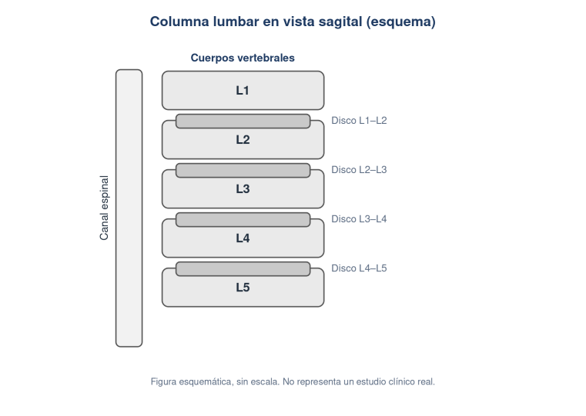
\includegraphics[width=0.92\textwidth]{images/anatomy/fig_c_01_columna_lumbar_sagital.png}
\caption{Esquema simplificado de vértebras lumbares, discos intervertebrales y canal espinal en vista sagital. Fuente: elaboración propia.}
\label{fig:anexo-c-columna-lumbar}
\end{figure}

\section{Esquema conceptual de segmentación.}

\begin{figure}[H]
\centering
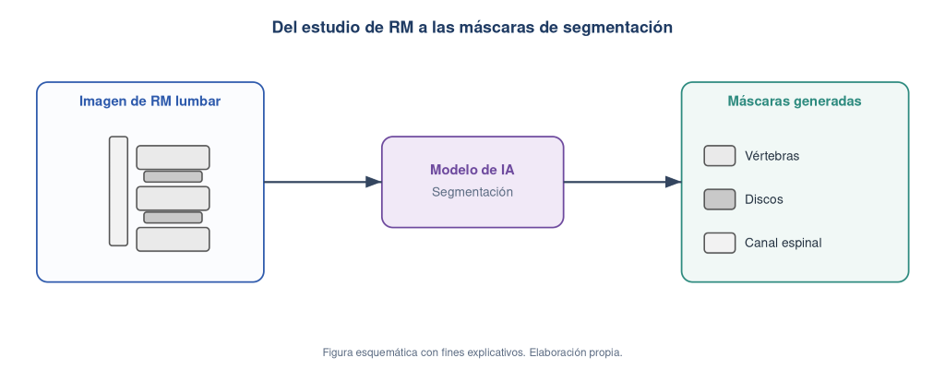
\includegraphics[width=0.92\textwidth]{images/anatomy/fig_c_02_segmentacion_conceptual.png}
\caption{Esquema conceptual del pasaje desde una RM lumbar hacia máscaras de segmentación. Fuente: elaboración propia.}
\label{fig:anexo-c-segmentacion-conceptual}
\end{figure}
